\documentclass[tikz,border=2pt]{standalone}
\usepackage{amsmath,amssymb}
\usepackage{tikz}
\usetikzlibrary{arrows.meta}

\begin{document}
% LP relaxation of a small integer program: the integer points (dots) are the true feasible
% set, the shaded polygon is the relaxation; its optimum (3.5, 1.25) is fractional and gives
% an upper bound 13 on the integer optimum 11 at (3, 1).
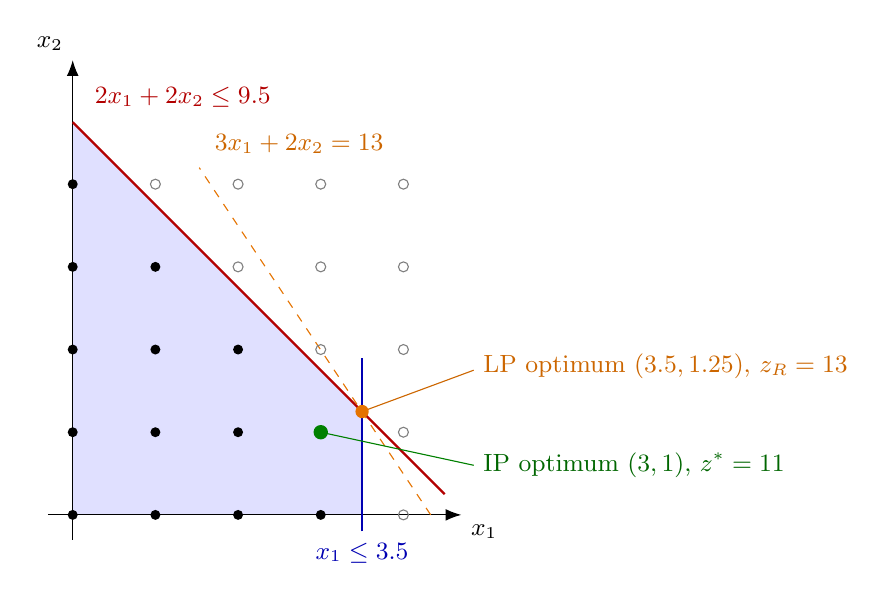
\begin{tikzpicture}[x=1.05cm, y=1.05cm, every node/.style={font=\small}, >={Latex[length=2mm]}]
	\fill[blue!12] (0,0) -- (3.5,0) -- (3.5,1.25) -- (0,4.75) -- cycle;
	\draw[->] (-0.3,0) -- (4.7,0) node[below right] {$x_1$};
	\draw[->] (0,-0.3) -- (0,5.5) node[above left] {$x_2$};
	\draw[blue!70!black, thick] (3.5,-0.2) -- (3.5,1.9);
	\draw[red!70!black, thick] (4.5,0.25) -- (0,4.75);
	\node[blue!70!black, font=\small, anchor=north] at (3.5,-0.22) {$x_1\le3.5$};
	\node[red!70!black, font=\small, anchor=west] at (0.15,5.05) {$2x_1+2x_2\le9.5$};
	\draw[orange!90!black, dashed] (4.33,0) -- (1.53,4.2);
	\node[orange!80!black, font=\small, anchor=south west] at (1.6,4.25) {$3x_1+2x_2=13$};
	\foreach \i in {0,1,2,3,4} {\foreach \j in {0,1,2,3,4} {
		\pgfmathparse{(2*\i+2*\j<=9.5 && \i<=3.5) ? 1 : 0}
		\ifnum\pgfmathresult=1 \fill[black] (\i,\j) circle (1.8pt); \else \draw[gray] (\i,\j) circle (1.8pt); \fi
	}}
	\draw[orange!80!black, thin] (3.5,1.25) -- (4.85,1.75);
	\draw[green!50!black, thin] (3,1) -- (4.85,0.6);
	\fill[orange!90!black] (3.5,1.25) circle (2.4pt);
	\fill[green!50!black] (3,1) circle (2.6pt);
	\node[orange!80!black, font=\small, anchor=west] at (4.85,1.8) {LP optimum $(3.5,1.25)$, $z_R=13$};
	\node[green!40!black, font=\small, anchor=west] at (4.85,0.6) {IP optimum $(3,1)$, $z^\ast=11$};
	\end{tikzpicture}
\end{document}
